
\documentclass[11pt]{article}


\usepackage{hyperref}
\usepackage{listings}
\usepackage{xcolor}


\usepackage{listings}
\usepackage{color}

\definecolor{codegreen}{rgb}{0,0.6,0}
\definecolor{codegray}{rgb}{0.5,0.5,0.5}
\definecolor{codepurple}{rgb}{0.58,0,0.82}
\definecolor{backcolour}{rgb}{0.95,0.95,0.92}


\lstset{frame=tb,
	backgroundcolor=\color{white},   
	commentstyle=\color{codegreen},
	keywordstyle=\color{magenta},
	numberstyle=\tiny\color{codegray},
	stringstyle=\color{codepurple},
	basicstyle=\footnotesize,
	breakatwhitespace=false,         
	breaklines=true,                 
	captionpos=b,                    
	keepspaces=true,                 
	numbers=left,                    
	numbersep=5pt,                  
	showspaces=false,                
	showstringspaces=false,
	showtabs=false,                  
	tabsize=2
}
\lstset{language=sh}

\usepackage{subfig}
\usepackage[utf8]{inputenc} % Required for inputting international characters
\usepackage[T1]{fontenc} % Output font encoding for international characters
\usepackage[margin=1.25in]{geometry}
\usepackage{mathpazo} % Palatino font
\usepackage{array}
\usepackage{float}
\usepackage{graphicx}
\usepackage{hyperref}
\usepackage{pdfpages}
\usepackage{natbib}
\setcounter{tocdepth}{2}
\graphicspath{ {C:/Users/Silvi/OneDrive/Desktop/Robotics/images} }

\usepackage{fancyhdr}
\usepackage[parfill]{parskip}
\pagestyle{fancy}

\begin{document}
				
		%configuring the header and footer here
		\fancyhead{} % clear all header fields
		\fancyhead[RO,LE]{\textbf{M00702000}}
		\fancyhead[LO,LE]{\textbf{Interim Report}}
		\fancyfoot{} % clear all footer fields
		\fancyfoot[CO]{\thepage}
		%Header and footer configuration ends here
		\begin{titlepage}	
			\centering
			
			\newcommand{\HRule}{\rule{\linewidth}{0.7mm }} % Defines a new command for horizontal lines, change thickness here
			\newcommand{\Botline}{\rule{\linewidth}{0.4mm }} % Defines a new command for horizontal lines, change thickness here
			
			
			
\includegraphics[width=0.5\linewidth]{mdx1.jpg}
			%		\textsc{\LARGE Institution Name}\\[1.5cm] % Main heading such as the name of your university/college
			
			\textsc{\Large Project Proposal }\\[0.5cm] % Major heading such as course name
			
			\textsc{\large Coursework 1}\\[0.5cm] % Minor heading such as course title
			
			%------------------------------------------------
			%	Title
			%------------------------------------------------
			
			\HRule\\[0.4cm]
			
			{\huge\bfseries Designing And Evaluating The Deployment Of A Mosquito Zapper Robot}\\[0.4cm] % Title of your document
			
			\Botline\\[1.5cm]
			
			%------------------------------------------------
			%	Author(s)
			%------------------------------------------------
			
			\begin{minipage}{0.4\textwidth}
				\begin{flushleft}
					\large
					\textit{Author}\\
					Silvia Aminul 
				\end{flushleft}
			\end{minipage}
			~
			\begin{minipage}{0.4\textwidth}
				\begin{flushright}
					\large
					\textit{Tutor}\\
					Dr. Tao Geng  
				\end{flushright}
				
				
			\end{minipage}
			
			
			\vfill\vfill\vfill
			
			\vfill
			%  	{\bfseries The author of this proposal \\  }
			
			
			
			{\bfseries M00702000 }
			\vfill
			{\large\today}
	\end{titlepage}
	\newpage
	\tableofcontents
	  
	
	
	\newpage
	\section{Introduction}
	
	The reliance on technology surges as the population of mosquitoes increase, this is becoming a growing public health concern as mosquitoes are known to carry a vast amount of diseases and rapidly transmit amongst humans and animals leading to severe illnesses and millions of deaths every year. Mosquitoes who are carrier of diseases are life threatening to those who are immunocompromised or have weakened immune systems.
	
	
	As the populations of mosquitoes increase so do the bites, their biotic %\cite{https://www.ncbi.nlm.nih.gov/pmc/articles/PMC1920178/}
	 interactions can especially imbalance the ecosystem as they play a major role on other species, from a holistic perspective their invasive nature can lead to drastic consequences on the environment, native species, and potentially human activities.
	 
	 	This project proposal aims to deliver an extensive overview on the execution of a robotic device that can eliminate high-powered mosquitoes through a laser beam upon detection using a high-resolution camera. 
	
	
		\section{Concept Behaviour}
	The Robot designed for this proposal will be able to do the with the following:
	\begin{itemize}
		\item To locate a mosquito without any external interventions (ex. human) this can be done through the aid of a advanced algorithms and sensors that finds the best way to kill them. 
		\item An imaging system can be placed above the robot to visualise its surrounding and identify mosquitoes through object recognition.
		\item Advanced sensors that can detect the presence of mosquitoes by their size, shape, movement, or other characteristics
		\item sensors to  stop robot from crashing into object and preventing external damages for example stopping if an object or human is in the way 
		\item Motors to allow the robot to move around in search of mosquitoes.
		\item A laser that can eliminate mosquitoes.
		\item to allow the camera face any direction a motor will be installed.
		\item to allow the laser point in any direction a motor will be installed.
		\item a source of power to help 
		\item A battery will be required as the power source in order to operate the robot for a long period of time.
		\item For the robot to operate autonomously a control system is required whereby human input is not required.
		\item to gradually improve the robots performance a machine learning algorithm will be implemented
		
	\end{itemize}
	
	
	\section{Background Research}
In this section will review that robots in the market that are similar in concept. This section will also include examining the different approaches taken to build a mosquito zapper  in research papers.
 	\subsection{LeiShen's Mosquito Zapper}
 	  \begin{center}
 	\begin{figure}[H]
 		\centering
 		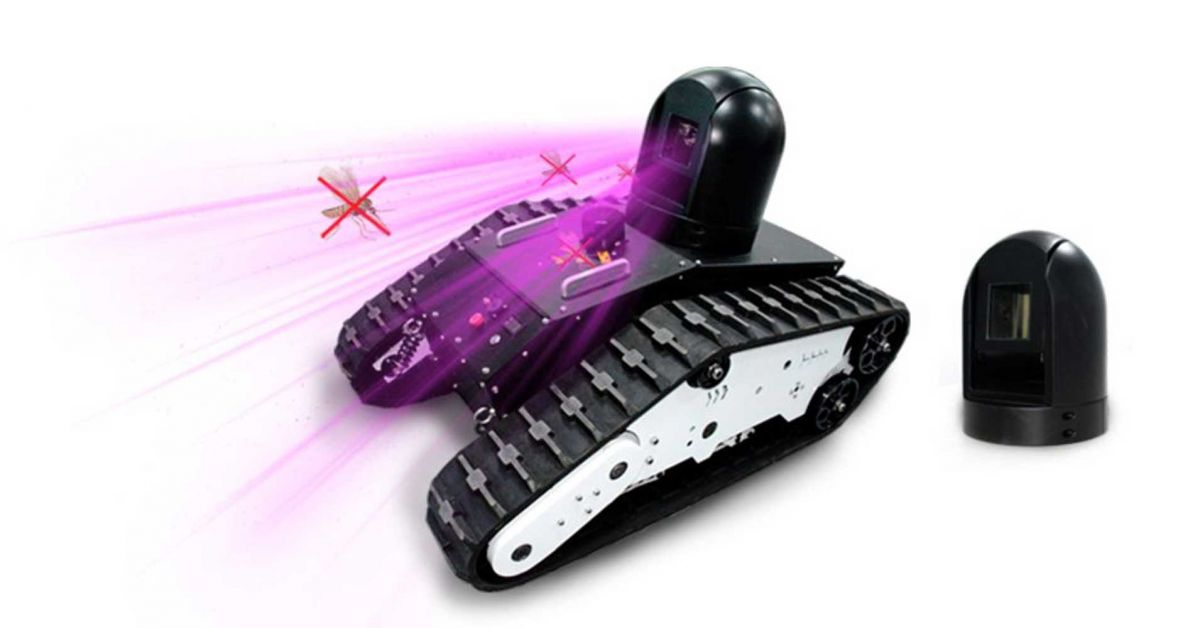
\includegraphics[width=0.8\linewidth]{robot.jpg}
 		
 	\end{figure}
 \end{center}
 
 This robot has been referred to as a toy-sized autonomous mosquito zapper, designed by a company named LeiShen. Although there is not much information on this whether this robot has actually been deployed or what kind of components it uses, this robot is similar to the project's aim.


\subsection{Autonomous Roomba}
  \begin{center}
	
	
	\begin{figure}[H]
		\centering
		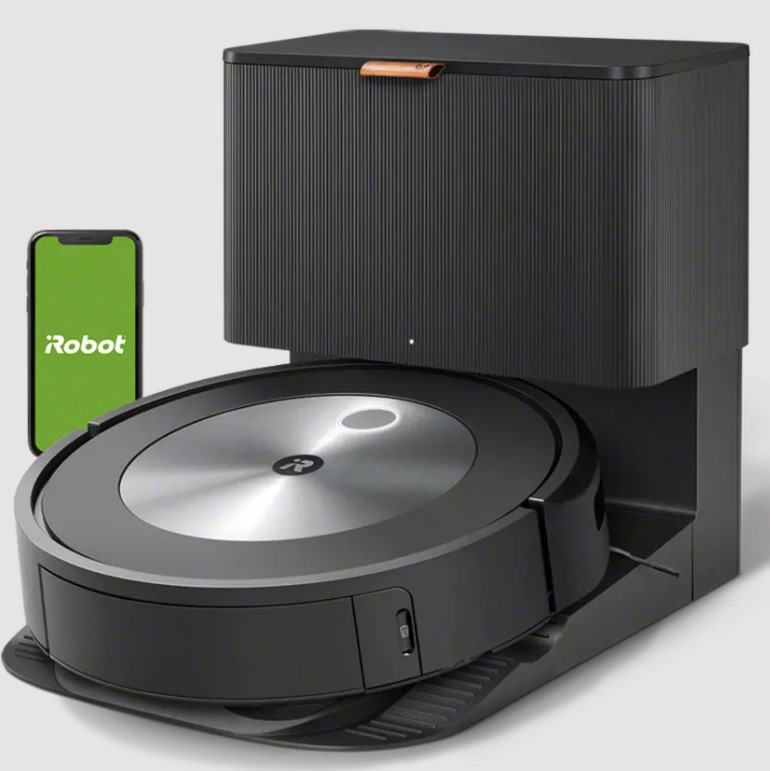
\includegraphics[width=0.46\linewidth]{robot2.jpg}
		
		\label{fig:Robot}
	\end{figure}
\end{center}

Although a robot vacuum is different from a mosquito zapper the concept is similar. This mosquito zapper should be able to roam around room autonomously just like the vacuum and avoid obstacles or have a hard encasing to control damage on the hardware. It 
\section{Challenges}
\subsection{OpenCV}

 In one similar experiment, it was found that using OpenCV solely to using a tracker function to track the movement of a mosquito in different methods did not give the greatest results. 
 \begin{center}
 	
 	
 	\begin{figure}[H]
 		\centering
 		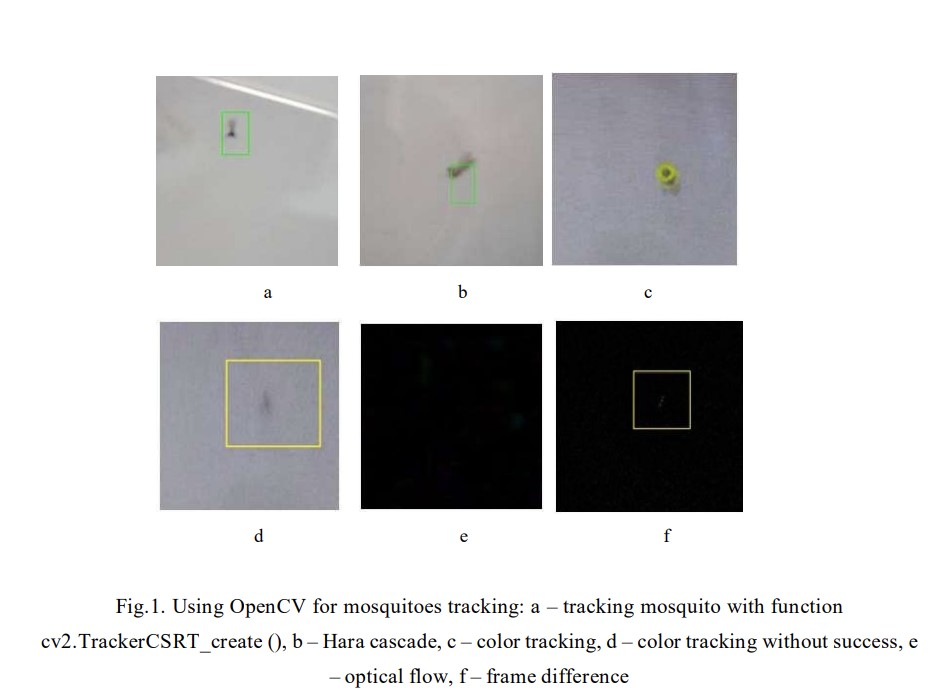
\includegraphics[width=1\linewidth]{opencv.jpg}

 		\label{fig:opencv}
 	\end{figure}
 \end{center}
 As seen in the figure above the mosquito in one of the methods cannot be detected at all, however by using an image processing function called Thresholding ON A 2-4mm sized mosquitoes gave drastically different results:\cite{rakhmatulin_2021_raspberry}
 
  
 \begin{center}
 	
 	
 	\begin{figure}[H]
 		\centering
 		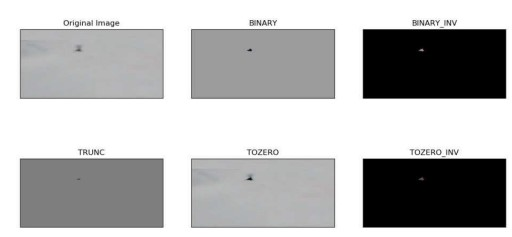
\includegraphics[width=0.8\linewidth]{opencv1.jpg}
 	
 		
 	\end{figure}
 \end{center}
 
 
 

 	
 \subsection{Design}
 
 
 
 
 
 	\section{Hardware structure}
 	 
 	
 	\begin{center}
 		
 		
 		\begin{figure}[H]
 			\centering
 			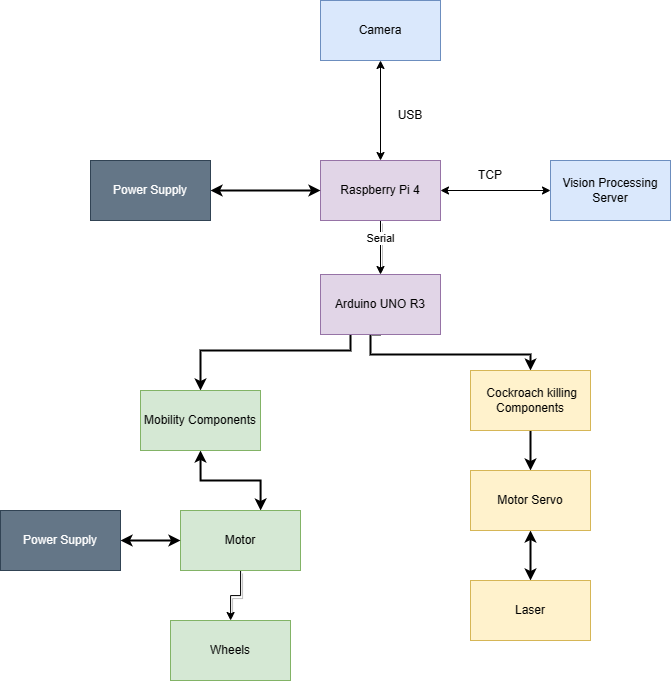
\includegraphics[width=1\linewidth]{hard.drawio.png}
 			\caption{An autonomous mosquito zapper robot roaming }
 			\label{fig:robot}
 		\end{figure}
 	\end{center}
 
 Components requiring to carry out high level task have either User Datagram Protocol (UDP) connection or Gigabit Ethernet, this is to minimise the risk of loosing importance of data due to the speed, if the perception component which is the initialising component  fails to deliver the right data on time it makes the robot ineffective at detecting the mosquito hence unable to annihilating mosquitoes, however UDP allows missing packets given this is not a viable option when detection small moving mosquitoes the better option for the camera is Gigabit Ethernet. TCP on the other hand is slightly lenient as although it is a slower method of sending data it is guaranteed that the data will be received, this form of connection has been used towards the lower level tasks such a movement and eliminating mosquitoes.
 
 
 
 In this project single boards will be used to control components. Jetson Nano can be used for the vision component (Camera), this single board has be chosen as its overall performance is better than most other computers, this is especially important if high resolution and excellent detection performance is required. The connection between the components was decided based on efficiency and requirement, Gigabit Ethernet has been used for two reasons, one of them being less latency. Reduced latency rates range from 5 to 20 ms and can stream a 4K content at a higher frame rate. 
 	\begin{center}
 	\setlength{\tabcolsep}{10pt} % Default value: 6pt
 	\renewcommand{\arraystretch}{1.5} % Default value: 1
 	\begin{tabular}{ | m{3cm} |m{3cm} | m{4cm}|  } 
 		
 			\hline
 		& Jetson Nano & Raspberry Pi 3A+   
 		\\ 
 		
 		\hline
 		
 		 GPU & 128-core NVIDIA Maxwell & Broadcom VideoCore IV  \\ 
 		
 		\hline
CPU
 		& 1.4 GHz 64-bit Quad-Core ARM Cortex-A57 MPCore & 1.4 GHz 64-bit quad-core ARM Cortex-A53
 		
 		\\ 
 		\hline
 		
 		
 		\hline
 RAM
 
 
 & 4GB LPDDR4 &
 512MB LPDDR2 SDRAM
 
 \\ 
 \hline
 		
 	Video Output: & HDMI, DisplayPort (4K) & HDMI, Display Serial Interface (DSI)
 		\\ 
 		\hline
 		Camera Serial Interface (CSI) & Yes & Yes\\ 
 		\hline
 		
 		
 		
 		\hline
 		Price (CSI) & £154.50 & £54.99\\ 
 		\hline
 	\end{tabular}
 \end{center}



For the central computer, Raspberry Pi 4 will be used as an affordable option as although its purpose is to carry out high level planning it does not require to use a lot of resources to carry out tasks.


Lastly the microcontroller, the series STM32F4, provides a range in terms of needs, it can provide sufficient memory to have excellent performance in terms of motion control.The STM32F407/417 product lines provide from 512 Kbytes to 1 MByte of Flash, 192 Kbytes of SRAM, and from 100 to
176 pins in packages as small as 10 x 10 mm. It's good performance, power efficiency and rich connectivity is the reason for choosing this microcontroller.



 \subsection{Simultaneous localization and mapping}
 	There are three steps in making a model functioning when implementing Simultaneous localization and mapping (SLAM) :
 \begin{itemize}
 	\item Perception - To achieve a model of the environment in which the robot will navigate in sensory components such as Lidar can be used, to do detect the mosquito a camera can be used with openCV. An ultrasonic sensor will be used in the case that the Lidar fails, this type of sensor is deemed useful if the object's vicinity is close.
 	\item Planning - consist planning how the autonomous interaction between the computers are going to take place without human interaction, to achieve this a high level central computer is going to be used to do high level planning and receive interfaces from the implementation of perception (Lidar and Camera). 
 	\item Action - Low level controllers is going to be used to control the encoders to move around the mapped environment and change the angle as well as direction of the laser.
 \end{itemize}
 \subsection{Key Hardware Components }
 \begin{itemize}
 	\item 	A high resolution camera is required to detect the size of a mosquito averaging the size of 2 to 4 mm, to configure this camera it must be ensured that the view from where the camera is placed is  clear and allows a wide view of the field where mosquitoes are most likely to be. The preferred frame rate per second should be 60, meaning the  roughly one image per every 16 ms should be coming through. Given only one computer is invested to solely receive data from the camera to process the image, a fast and high quality computer such as the Jetson Nano Computer should be fast enough to process the frames.
 	
 	\item A laser strong enough to neutralise a mosquito however weak enough to not harm the human eye is required to make this robot safer, to configure the laser according the camera's coordinates the laser can be attached to a Servo motor before it is fixed on the robot.
 	
 	\item A motor servo would be controlled though the microcontroller (STM32F4) which receives information from the main control system (Raspberry Pi 4),using the location and movement provided by the Jetson Nano.To make the laser move according to the camera, a servo can be used or in a scaled up project robotic arm to aim the laser. In this case the servo motor can be controlled by the robot's control system,  using the location and movement information of the detected mosquitoes provided by the camera and image processing algorithms.
 	
 	
 	
 	
 \end{itemize}
 
 	 	\subsection{Steps in Connecting the Hardware}
 	 	
 	 	The camera and sensors (Ultrasonic sensor for obstacle avoidance) can be connected to the control system with the  right cables, upon receiving a location and movement information input the control system can use the data to adjust the robots movement and adjust the laser's aim.
 	
 	When executing this project a decision must be made on what type component should be used to reposition the laser's aim when a mosquito is detected. One can use a servo motor or a robotic arm, in this project the proposed component is a servo motor.
 	
 	


 The laser connected to the servo motor or robotic arm should then be connected to the control system with the right cables, the purpose of the laser is aim and kill mosquitoes detected from a calculated direction from the coordinates received from the camera.
 
 To ensure the system is working the circuit should be tested at this point and make further adjustments.
 	One adjustment required will be the calculation of the laser's's aim when pointing at the mosquito, this is going to be dependant on the robot's design in terms of size and distance from the camera. To detect mosquitoes the camera is going to use image processing function, given the placement of the laser and the camera  on the chassis is going to be different from each other, the camera's coordinates on the detected mosquitoes is not going to allow the laser to aim correctly, therefore an angle direction will be need to be adjusted in the servo motor to point the laser correctly.
 	
 	
 	To calculate this, the angle at which the servo motor needs to move the laser is required. This can be done using basic trigonometry, by calculating the angles formed by the lines connecting the center of the camera's field of view, the location of the detected mosquito, and the servo motor axis.
 	
 	Alternatively, if the robot uses a robotic arm to aim the laser, the location of the detected mosquito in three-dimensional space  can be used to calculate the position and orientation of the end effector (the part of the robotic arm that holds the laser) that is required to point the laser at the mosquito. This can be done using inverse kinematics algorithms, which calculate the joint angles of the robotic arm that are necessary to achieve a desired end effector position and orientation.
 	

 
 \section{Software}
 
 \begin{center}
 	
 	
 	\begin{figure}[H]
 		\centering
 		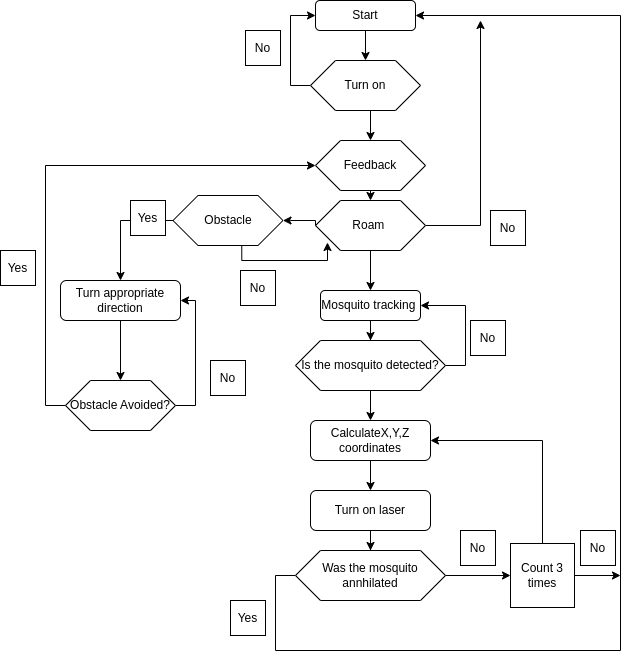
\includegraphics[width=0.8\linewidth]{flaw.drawio.png}
 		\caption{A flowchart  }
 		\label{fig:Flowchart}
 	\end{figure}
 \end{center}
 

AN image processing algorithm such opencv though raspberry pi can be used  to automatically detect and track mosquitoes in the camera's field of view. This can be done using techniques such as thresholding, edge detection, and object recognition algorithms.

The detected mosquitoes can be used to identify their location and movement direction, and use this information to control the robot's movements and aim the laser.

Once detected and in close range to the mosquito the lase can be then used to fire at the detected mosquitoes, using the robot's aiming mechanism, to kill them on contact.


To make the laser move according to the camera, a servo can be used or in a scaled up project robotic arm to aim the laser. In this case the servo motor can be controlled by the robot's control system, using the location and movement information of the detected mosquitoes provided by the camera and image processing algorithms.

For instance,if the control system uses the location of the detected mosquitoes to calculate the necessary angle and direction for the servo motor or robotic arm to move the laser, this information can then be sent to the servo motor or robotic arm, which will move the laser to the desired position.

Alternatively, a fixed laser and position the camera and servo motor or robotic arm in such a way that the laser is always aimed at the center of the camera's field of view. In this case, the control system can use the movement of the detected mosquitoes to adjust the pan and tilt angles of the camera and servo motor or robotic arm, to keep the laser pointed at the mosquitoes as they move.

Overall, the key to making the laser move according to the camera is to use a control system that can process the location and movement information of the detected mosquitoes, and use this information to control the servo motor or robotic arm that aims the laser.








	

	
	

	\section{Component List}

		
	
	\textbf{High-resolution cameras} or a specialized sensor that can detect the presence of mosquitoes. A camera with a high frame rate and good resolution can be used to capture images of mosquitoes and identify them based on their shape and size. This can be combined with image processing algorithms to automatically detect and track mosquitoes in real-time.
	
	
		 \begin{center}
		
		
		\begin{figure}[H]
			\centering
			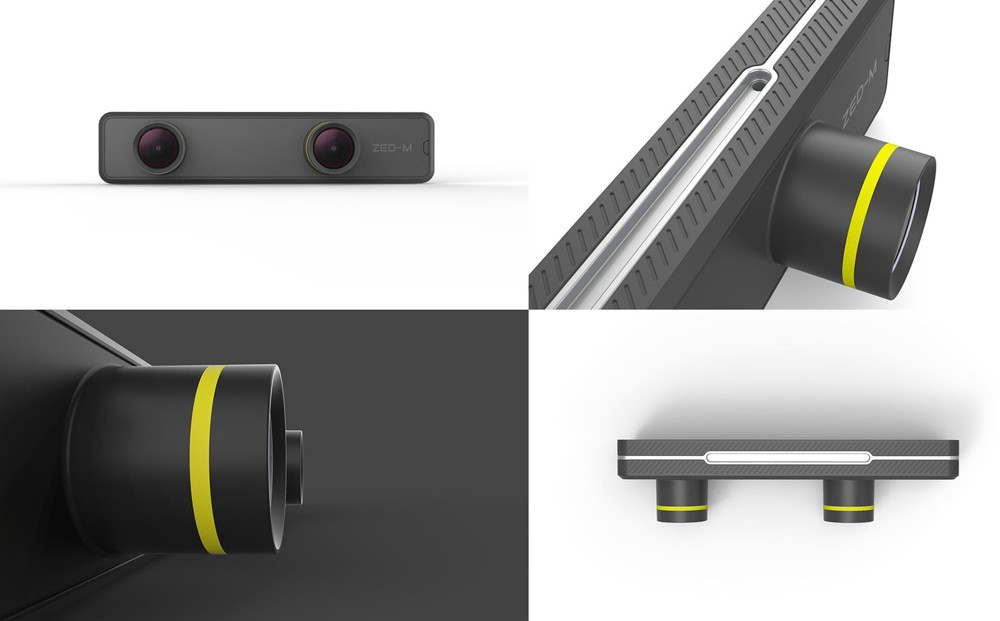
\includegraphics[width=0.5\linewidth]{zed.jpg}
			\caption{High-resolution camera: A Stereo Camera such as the Zed Mini can be used to detect and track mosquitoes in the robot's field of view.}  
			\label{fig:Flowchart}
		\end{figure}
	\end{center}
	
	

	
		\textbf{Servo motor or robotic arm}: A servo motor, such as the Tower Pro SG90 or the DYNAMIXEL AX-12A, can be used to aim the laser at the detected mosquitoes.	
	 \begin{center}
		
		
		\begin{figure}[H]
			\centering
			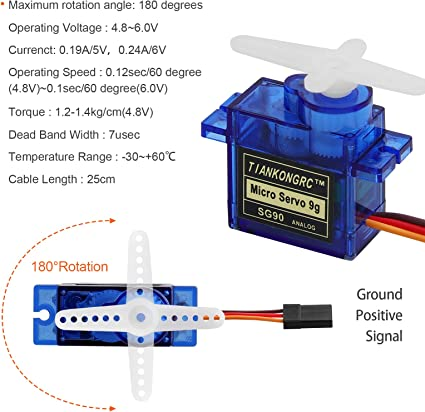
\includegraphics[width=0.5\linewidth]{motor.jpg}
			\caption{SG90 9g Micro Servos for RC Robot Helicopter Airplane Controls Car Boat}  
		\label{fig:Flowchart}
	\end{figure}
\end{center}
	
	
	
	\textbf{Laser}: A laser, such as the 445nm Blue Laser Module or the 532nm Green Laser Module, can be used to kill the detected mosquitoes on contact.	A laser, or other high-intensity light source, that is capable of killing mosquitoes on contact.
	
	 \begin{center}
		
		
		\begin{figure}[H]
			\centering
			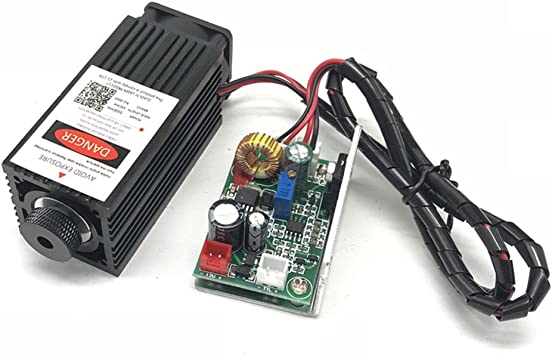
\includegraphics[width=0.5\linewidth]{laser.jpg}
			\caption{High Power 445nm Focusing Blue Laser Module Laser Engraving}  
			\label{fig:Flowchart}
		\end{figure}
	\end{center}
	
	\textbf{Control system}: A control system, such as a Raspberry Pi 4, can be used to process the input from the camera and other sensors, and control the servo motor or robotic arm and the laser.	A control system, such as a microcontroller or a computer, to process the input from the mosquito detection system and control the laser firing mechanism.
	
		 \begin{center}
		
		
		\begin{figure}[H]
			\centering
			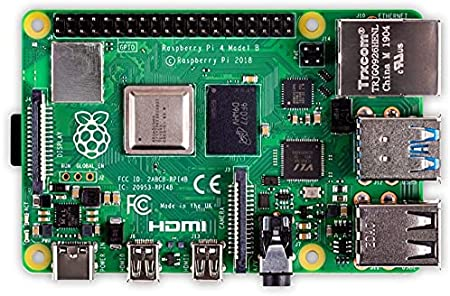
\includegraphics[width=0.5\linewidth]{ard.jpg}
			\caption{ Raspberry Pi 4 Model B 8GB }
			\label{fig:Flowchart}
		\end{figure}
	\end{center}

The decision of using following computers have been explained in the hardware section.
	 \begin{center}
	
	
	\begin{figure}[H]
		\centering
		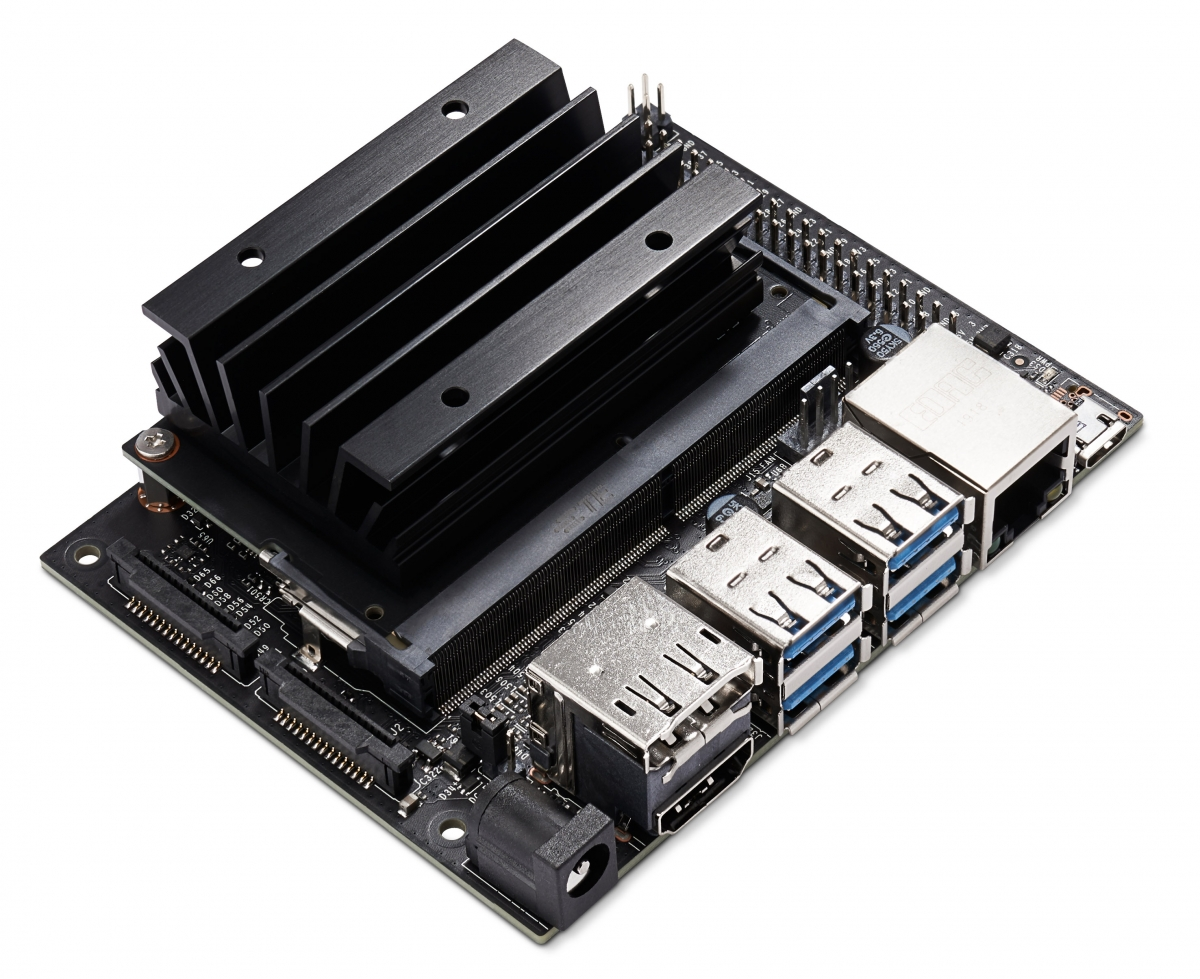
\includegraphics[width=0.5\linewidth]{jet.jpg}
		\caption{ Jetson Nano Developer Kit }
		\label{fig:Flowchart}
	\end{figure}
\end{center}
 \begin{center}
	
	
	\begin{figure}[H]
		\centering
		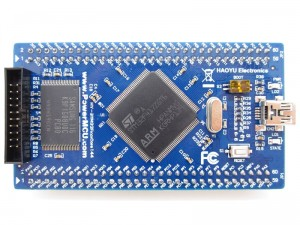
\includegraphics[width=0.5\linewidth]{stm.jpg}
		\caption{ST STM32F407/417 }
		\label{fig:Flowchart}
	\end{figure}
\end{center}




	
	\textbf{Power supply}: A power supply, such as a battery or a plug-in power supply, can be used to provide the necessary electrical energy for the circuit.
		A power source, such as a battery or a plug-in power supply, to provide the necessary energy for the laser and the other components.
	
	
	

	

	

	
\textbf{	A housing or chassis} to hold and protect the other components, and provide a way for the robot to move around and access areas where mosquitoes may be present.
	
	In addition to these core components, additional hardware and software components, such as sensors will be required for navigation and obstacle avoidance (SLAM), and software for image processing and control algorithms.
	
	
	
	


	

	
		\section{Safety Protocol}
	
	To make sure that mosquito annihilating robot is safe to operate, the following steps can be taken as precaution:
	\begin{itemize}
		\item 	Using appropriate wiring and connectors should ensure that the connection is strong and can be used with the appropriate voltage, there are few ways to notice faults which include if the wire is heating up there maybe a shortage one can check the readings on a multimeter and the components specification to get a better understanding, in another instance one motor maybe failing to work due to not enough volts, this can be checked using tools that allows checking how much voltage is enough to run both motors.
		\item 
		Although fuses have not been used in this project in a real scenario where this robot would be used as a household item, fuses or circuit breakers may be required to prevent potential hazardous malfunctions such as excessive current or a short circuit.
		\item To ensure the right voltage is being used in the circuit using appropriate power sup-plies and voltage regulators should be used to prevent hazardous situations, this can prevent potential damage within the components and ensure the robot is operating at its optimal.
		\item Using heat sinks and other cooling techniques should be able to prevent components from overheating, this can help components getting rid of excessive heat and operate components under safe temperature.
		\item And lastly the circuit must always be tested before operating to make sure the robot would function properly and safely.There's a variety of equipment available to test this including but not limited to multimeters.
		
		
		
	\end{itemize}
	

	
	
	
	
	


	
	
	\section{Further Development}
	

After the robot one issue remained with connecting the raspberry pi to the internet and reconfiguring the ip address, to fix this programming the the raspberry pi to automatically connect would make the setting up process a much faster.


More than one sensor can be used to detect mosquitoes more accurately, this can include:

Developing and using a more complex algorithms to detect mosquitoes, and track their movement, as the current robot does not track moving mosquitoes. Implementing a mosquito tracking robot that can detect mosquitoes in different kinds of environment  would make the robot more efficient and improve its detection accuracy.

Implementing obstacle avoidance by using LIDAR/SLAM or ultrasonic sensors may help the robot navigate without damaging itself would be make it suitable to operate in real environments where the are object and people. 

To further develop this robot, efficiency in terms of power usage can be looked at starting from adding solar panels to reserve energy in public settings, to developing a house the robot can go back when battery is low in a home setting. Adding such power management strategies would greatly enable for the robot to operate longer before having a human checking on its battery health.

Implementing other functions in this robot such as having a insecticide spray attached can help evolve further.

The following part of this section will look more into sensors that this robot can have:
\begin{itemize}
	\item Acoustic Sensors: mosquitoes make certain sounds that may require further research, if detetected by a microphone or an acoustic sensor, such a sensor can be used to detect the exact location of the sensor,if not, it can help verify its presence.
	
	\item Chemical sensors: Looking into the types of chemicals mosquitoes are attracted can be studied, examples of this can include lactic acid and other human perspiration compounds. A gas chromatograph which is a chemical sensor can be used to detect these certain chemical and infer the possibility of the presence of mosquitoes.
	\item 	Heat sensors: heat and CO2 transmitted by warm-blooded beings is something mosquitoes are quite attracted to therefore, implementing heat sensor such as thermal imaging camera should be considered to detect the mosquitoes though detecting heat signature. 
	\item 
	\item Advancement sensors: Can be used to prevent the robot from crashing into humans and prevent its externals from being damaged.
	\end{itemize}

	

	
	
	

	
	
	\section{Conclusion}
	
	
To conclude this proposal, many things have been considered, this robot may become a project that is scalable and put and end to the millions of deaths. Although this is just a proposal, this proposal as a project would require a lot more planning and changes. Therefore to achieve something similar at university level, a cockroach will be used which is an insect that is similar but at a ground level, in this case an accurate level of detection would be prioritised. Nonetheless, the concept of automating technology that deals with pests is more than necessary than ever before. 

	\section{References }
	
	\renewcommand{\bibsection}{}
	
	\bibliographystyle{unsrt}
	
	\bibliography{reference}
	
	
	
	\end{document}


